%================ch4======================================
\chapter{Conclusions}\label{ch:ch4}

A plot of the area between tracks and $N_{relax}$ was made and a regression line was fit to the data. The cluster IC 4651, the oldest cluster in the study, has undergone multiple relaxations having a rather short relaxation time of 41 million years. NGC 752 and IC 4756 are very likely to have some external bodies influencing their gravity which prevents them from settling. Both these clusters have the largest calculated relaxation times. The have many more single stars than binaries across the cluster giving both a very large negative area difference. Most of the other clusters in the bottom right of the plot seem to follow the trend. NGC 6405 is another outlier and this can be attributed to its very young age (90 million years). It has not even completed its first relaxation period yet has a somewhat mature structure. 

\begin{figure}[h]
	\centering
	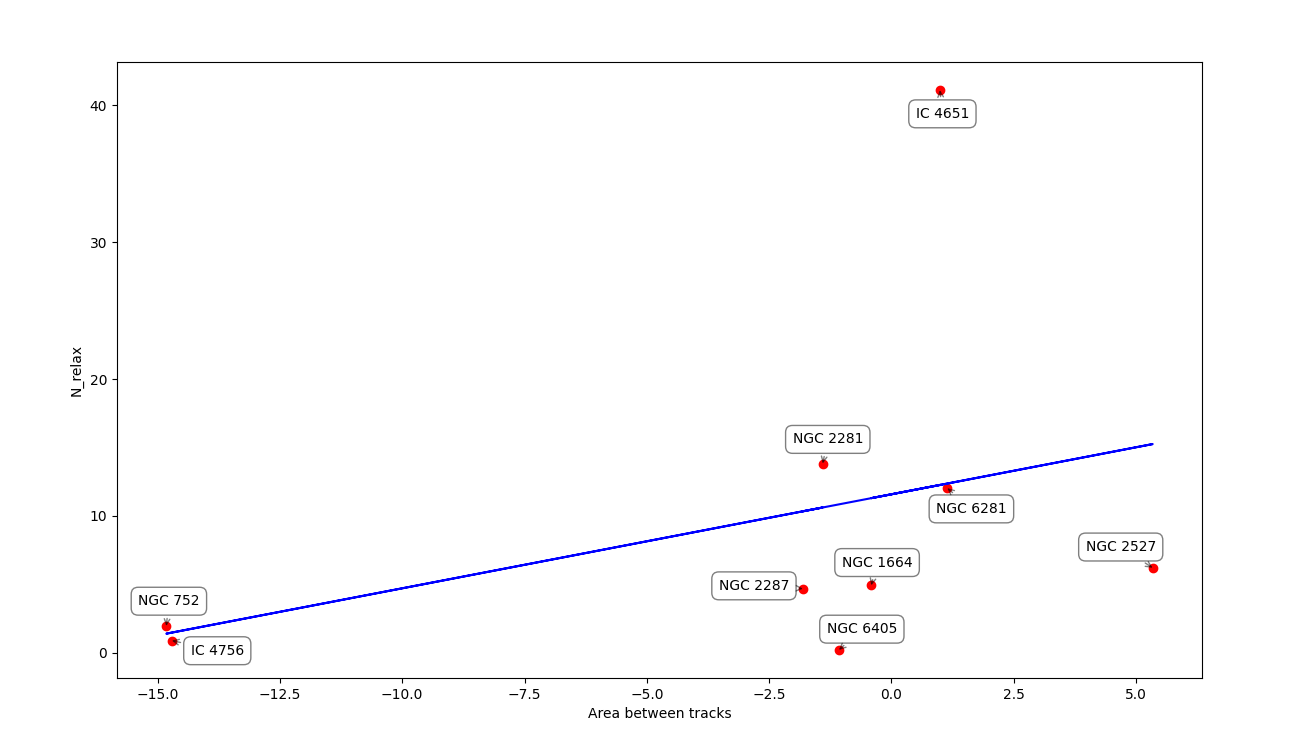
\includegraphics[width=\linewidth]{final_plot.png}
	\caption{The plot of area between tracks v $N_{relax}$}
	\label{fig:im8}
\end{figure}

The presence of far outliers and the large gap between the left and right ends indicates there is insufficient data for this study. Including more clusters might fill the gap. Performing the analysis for more clusters would also help determine if there is a correlation and improve its strength.